\documentclass[aspectratio=169]{beamer}
\usepackage[T1]{fontenc}
\usepackage[utf8]{inputenc}
\usepackage[ngerman]{babel}
\usepackage{amsmath,amssymb}
\usepackage{booktabs}
\usepackage{graphicx}
\usepackage{xcolor}

\usetheme{Madrid}
\usecolortheme{default}
\setbeamertemplate{navigation symbols}{}

\definecolor{tuwblue}{RGB}{0,102,153}
\setbeamercolor{structure}{fg=tuwblue}
\setbeamercolor{title}{fg=white,bg=tuwblue}
\setbeamercolor{frametitle}{fg=white,bg=tuwblue}

\setbeamersize{text margin left=5mm, text margin right=5mm}

\title{Hess-Smith Panelverfahren}
\subtitle{Berechnung ebener Potentialströmungen um geschlossene Körper}
\author{Sebastian Matkovich}
\institute{TU Wien}
\date{2026}

\newcommand{\plotimg}[1]{\includegraphics[width=\textwidth,height=2.8cm,keepaspectratio]{#1}}

\begin{document}

\begin{frame}
  \titlepage
\end{frame}

%=== FOLIE 1: Problemstellung ===
\begin{frame}{Problemstellung}
\footnotesize

\begin{columns}[T]
\begin{column}{0.55\textwidth}
Berechnung der Druckverteilung und des
Auftriebs an Tragflächenprofilen mittels des
\textbf{Hess-Smith Panelverfahrens}.

\begin{enumerate}\setlength\itemsep{2pt}
  \item Implementierung in MATLAB
  \item Validierung am Kreiszylinder (analytische Lösung)
  \item Anwendung auf Tragflächenprofile
  \item Vergleich mit XFOIL (Referenz)
\end{enumerate}

\medskip
\textbf{Untersuchte Profile} (UIUC-Datenbank):
\begin{itemize}\setlength\itemsep{1pt}
  \item NACA\,0012 -- symmetrisch
  \item Eppler\,193 \& 205 -- gewölbt
\end{itemize}
\end{column}
\begin{column}{0.42\textwidth}
  \vspace{-1mm}
  \plotimg{crop_004.png}
  \vspace{-1mm}
  {\tiny\centering NACA\,0012 -- symmetrisch\par}
  \vspace{2mm}
  \plotimg{crop_002.png}
  \vspace{-1mm}
  {\tiny\centering Eppler\,193 -- gewölbt\par}
\end{column}
\end{columns}

\end{frame}

%=== FOLIE 2: Annahmen → Laplace ===
\begin{frame}{Physikalische Grundlagen -- Laplace-Gleichung}
\footnotesize

\textbf{Annahmen:} ebene, stationäre, inkompressible, reibungsfreie Strömung.

\medskip
\begin{columns}[T]
\begin{column}{0.48\textwidth}
\textbf{1.\;Wirbelfreiheit} (Helmholtz):

\smallskip
Reibungsfrei $\Rightarrow$ $\nabla\times\vec{v}=0$

$\Rightarrow$ Geschwindigkeitspotential existiert: $\;\vec{v} = \nabla\varphi$
\end{column}
\begin{column}{0.48\textwidth}
\textbf{2.\;Kontinuitätsgleichung} (Massenerhaltung):
\vspace{-1mm}
\[
  \underbrace{\frac{\partial\rho}{\partial t}}_{=\,0\;\text{(stat.)}}
  +\;\nabla\cdot\bigl(\underbrace{\rho\vphantom{\frac{\partial}{\partial t}}}_{=\,\text{const}}\vec{v}\bigr) = 0
  \;\;\Longrightarrow\;\;
  \nabla\cdot\vec{v} = 0
\]
\end{column}
\end{columns}

\medskip
Einsetzen von $\vec{v}=\nabla\varphi$ in $\nabla\cdot\vec{v}=0$:
\vspace{-1mm}
\[
  \nabla\cdot(\nabla\varphi) = \Delta\varphi = 0
  \qquad\text{-- die \textbf{Laplace-Gleichung}}
\]

\vspace{-2mm}
Weil sie \textbf{linear} ist, erfüllt jede Überlagerung von Lösungen sie ebenfalls.
$\to$ Idee: Körperkontur in $n$ \textbf{Panele} unterteilen, auf jedem eine Quellverteilung
ansetzen -- $\Delta\varphi=0$ ist automatisch erfüllt, nur die Randbedingung bleibt.

\end{frame}

%=== FOLIE 3: Elementarlösung ===
\begin{frame}{Elementarlösung -- Die Punktquelle}
\footnotesize

\begin{columns}[T]
\begin{column}{0.48\textwidth}
\textbf{Radialsymmetrischer Ansatz} $\varphi(r)$.

\smallskip
Laplace in Polarkoordinaten ohne $\theta$:
\vspace{-1mm}
\[
  \frac{1}{r}\frac{d}{dr}\!\left(r\frac{d\varphi}{dr}\right) = 0
\]

\vspace{-2mm}
Erste Integration: $\;r\,\varphi' = C_1$, also $\;\varphi' = C_1/r$.

Zweite Integration: $\;\varphi = C_1 \ln r + C_2$.

\medskip
\textbf{Bestimmung von $C_1$:} Der Volumenstrom durch
einen beliebigen Kreis um die Quelle muss gleich
der Quellstärke~$m$ sein.
\end{column}
\begin{column}{0.48\textwidth}
Mit $\vec{v}=\frac{C_1}{r}\hat{e}_r$,\; $\hat{n}=\hat{e}_r$,\; $ds=r\,d\theta$:
\vspace{-1mm}
\[
  \oint\vec{v}\!\cdot\!\hat{n}\;ds
  = \int_0^{2\pi}\!\frac{C_1}{r}\,r\,d\theta
  = 2\pi C_1 \stackrel{!}{=} m
\]

\vspace{-2mm}
$r$ kürzt sich -- gleicher Strom durch jeden Kreis.

$\Rightarrow\; C_1 = \tfrac{m}{2\pi}$

\medskip
\textbf{Ergebnis} -- Punktquelle mit Stärke $m$:
\vspace{-1mm}
\[
  \boxed{\varphi = \frac{m}{2\pi}\ln r\,,
  \qquad
  \vec{v} = \frac{m}{2\pi r}\,\hat{e}_r}
\]

\vspace{-2mm}
Radialsymmetrisches Feld, erfüllt $\Delta\varphi=0$.
\end{column}
\end{columns}

\end{frame}

%=== FOLIE 4: Vom Panel zum Integral ===
\begin{frame}{Von der Punktquelle zum Panel -- Einflusskoeffizienten}
\footnotesize

\begin{columns}[T]
\begin{column}{0.48\textwidth}
Auf Panel~$j$: kontinuierliche Verteilung von
Punktquellen mit konstanter Stärke~$q_j$ (pro Längeneinheit).
Jedes Stückchen $dl'$ trägt $dm\!=\!q_j\,dl'$ bei:
\vspace{-1mm}
\[
  \vec{v}_{ij} = q_j
  \underbrace{\int_{\text{Panel}\,j}
  \frac{1}{2\pi}\,
  \frac{\vec{r}_i - \vec{r}'}{|\vec{r}_i - \vec{r}'|^2}\,dl'}_{\text{nur Geometrie}}
\]

\vspace{-3mm}
Zur analytischen Auswertung: Transformation in das
\textbf{lokale Koordinatensystem} von Panel~$j$.
Das Panel liegt entlang der $\xi$-Achse von $-l_j/2$
bis $+l_j/2$, $\eta$ ist der Normalabstand:
\vspace{-1mm}
\begin{align*}
  \xi_{i,j} &= (X_i\!-\!X_j)\cos\theta_j + (Y_i\!-\!Y_j)\sin\theta_j \\[-1pt]
  \eta_{i,j} &= -(X_i\!-\!X_j)\sin\theta_j + (Y_i\!-\!Y_j)\cos\theta_j
\end{align*}
\end{column}
\begin{column}{0.48\textwidth}
In diesem System wird das Integral analytisch lösbar.
Ergebnis -- die geometrischen Integrale:
\vspace{-1mm}
\begin{align*}
  I_{i,j} &= \frac{1}{4\pi}\ln\frac{(l_j+2\xi)^2+4\eta^2}
                                     {(l_j-2\xi)^2+4\eta^2} \\[2pt]
  J_{i,j} &= \frac{1}{2\pi}\!\left[
    \arctan\frac{l_j-2\xi}{2\eta}
    + \arctan\frac{l_j+2\xi}{2\eta}\right]
\end{align*}

\vspace{-3mm}
\textbf{Einflusskoeffizienten} -- Rückdrehung ins globale
System und Projektion auf Panel~$i$:
\vspace{-1mm}
\begin{align*}
  A^{(n)}_{i,j} &= -\sin(\theta_i\!-\!\theta_j)\,I_{i,j}
                   +\cos(\theta_i\!-\!\theta_j)\,J_{i,j} \\[2pt]
  A^{(t)}_{i,j} &= +\cos(\theta_i\!-\!\theta_j)\,I_{i,j}
                   +\sin(\theta_i\!-\!\theta_j)\,J_{i,j}
\end{align*}

\vspace{-4mm}
$M_{i,j} = A^{(n)}_{i,j}$ -- so gehen die Panels in die Matrix ein.
\end{column}
\end{columns}

\end{frame}

%=== FOLIE 5: Geschwindigkeitsprojektion → LGS ===
\begin{frame}{Vom Einflusskoeffizienten zum Gleichungssystem}
\footnotesize

Die \textbf{Gesamtgeschwindigkeit} am Mittelpunkt von Panel~$i$ ist die
Überlagerung aller Panelbeiträge plus der Anströmung:
\vspace{-1mm}
\[
  \vec{v}_i = \vec{V}_\infty + \sum_j \vec{v}_{ij}
\]

\vspace{-3mm}
\begin{columns}[T]
\begin{column}{0.48\textwidth}
\textbf{Normalkomponente} -- wird zu null gesetzt
(\textbf{Undurchlässigkeitsbedingung}):
\vspace{-1mm}
\[
  \underbrace{V_\infty\sin(\alpha\!-\!\theta_i)}_{\text{Anströmung}}
  + \underbrace{\sum_j A^{(n)}_{i,j}\,q_j}_{\text{alle Panels}}
  \stackrel{!}{=} 0
\]

\vspace{-2mm}
Das sind $n$ Gleichungen für $n$ Unbekannte $q_j$:
\vspace{-1mm}
\[
  \boxed{M\,\vec{q} = \vec{b}}
  \quad\text{mit}\;
  b_i = -V_\infty\sin(\alpha\!-\!\theta_i)
\]
\end{column}
\begin{column}{0.48\textwidth}
\textbf{Tangentialkomponente} -- auswerten mit
bekannten $q_j$ (\emph{keine} Gleichung, nur einsetzen):
\vspace{-1mm}
\[
  v_{t,i} =
  \underbrace{V_\infty\cos(\alpha\!-\!\theta_i)}_{\text{Anströmung}}
  + \underbrace{\sum_j A^{(t)}_{i,j}\,q_j}_{\text{alle Panels}}
\]

\vspace{-2mm}
$\alpha\!-\!\theta_i$ ist der Winkel zwischen Anströmung
und Paneltangente:
\begin{itemize}\setlength\itemsep{0pt}
  \item $\sin$ projiziert auf \textbf{Normale} (senkrecht)
  \item $\cos$ projiziert auf \textbf{Tangente} (parallel)
\end{itemize}
\end{column}
\end{columns}

\end{frame}

%=== FOLIE 6: Bernoulli → cp ===
\begin{frame}{Vom $v_t$ zum Druckbeiwert $c_p$}
\footnotesize

\textbf{Bernoulli} entlang einer Stromlinie zwischen ungestörter Anströmung und Oberfläche:

\begin{columns}[T]
\begin{column}{0.48\textwidth}
\[
  p_\infty + \tfrac{1}{2}\rho\, V_\infty^2
  \;=\;
  p + \tfrac{1}{2}\rho\, v_t^2
\]

Umstellen nach der Druckdifferenz:
\[
  p - p_\infty = \tfrac{1}{2}\rho\bigl(V_\infty^2 - v_t^2\bigr)
\]

Normieren auf den dynamischen Druck $\tfrac{1}{2}\rho V_\infty^2$:
\[
  \boxed{c_p \;=\; \frac{p - p_\infty}{\tfrac{1}{2}\rho\,V_\infty^2}
  \;=\; 1 - \left(\frac{v_t}{V_\infty}\right)^{\!2}}
\]
\end{column}
\begin{column}{0.48\textwidth}
\textbf{Interpretation:}

\medskip
\begin{itemize}\setlength\itemsep{4pt}
  \item $V_\infty$ -- Anströmgeschwindigkeit\\
        (ungestört, weit vom Körper)
  \item $v_t$ -- Tangentialgeschwindigkeit am Panel\\
        (Normalkomponente $= 0$ auf Oberfläche)
  \item $c_p = 1$: \textbf{Staupunkt} ($v_t = 0$)
  \item $c_p < 0$: \textbf{Sog} ($v_t > V_\infty$)
  \item $c_p = 0$: lokale Geschwindigkeit $= V_\infty$
\end{itemize}
\end{column}
\end{columns}

\medskip
\textbf{Zusammenfassung Rechenweg:}\;
Profildaten $\to$ Panele $\to$ $M\vec{q}=\vec{b}$ lösen $\to$ $v_{t,i}$ berechnen $\to$ $c_p$

\end{frame}

%=== FOLIE 7: Zylinder — Analytische Lösung ===
\begin{frame}{Validierung am Kreiszylinder -- Analytische Lösung}
\footnotesize

\begin{columns}[T]
\begin{column}{0.57\textwidth}
Überlagerung Parallelströmung + Dipol:
\vspace{-1mm}
\[
  \varphi = V_\infty\!\left(r + \frac{R^2}{r}\right)\cos\theta
\]

\vspace{-3mm}
Radialgeschwindigkeit bei $r\!=\!R$: $\;v_r = V_\infty\!\left(1-\frac{R^2}{r^2}\right)\cos\theta \xrightarrow{r=R} 0\;\checkmark$

\smallskip
Tangentialgeschwindigkeit bei $r\!=\!R$:
\vspace{-1mm}
\[
  v_t = -2V_\infty\sin\varphi
\]

\vspace{-3mm}
Einsetzen in $c_p = 1-(v_t/V_\infty)^2$:
\vspace{-1mm}
\[
  c_p = 1-4\sin^2\!\varphi
  \;\;\xrightarrow{\sin^2\!=\,\frac{1-\cos 2\varphi}{2}}\;\;
  c_p = 2\cos(2\varphi)-1
\]

\vspace{-3mm}
\begin{itemize}\setlength\itemsep{0pt}
  \item $\varphi\!=\!0^\circ,\,180^\circ$: Staupunkte ($c_p\!=\!1$)
  \item $\varphi\!=\!90^\circ$: $c_p\!=\!-3$ (Maximum der Geschwindigkeit)
\end{itemize}

\textbf{D'Alembertsches Paradoxon:} symm.\ Druck $\Rightarrow$ kein Widerstand.
\end{column}
\begin{column}{0.40\textwidth}
  \vspace{-1mm}
  \plotimg{crop_005.png}
  \vspace{-1mm}
  {\tiny\centering 8 Panels -- grobe Näherung\par}
  \vspace{2mm}
  \plotimg{crop_006.png}
  \vspace{-1mm}
  {\tiny\centering 32 Panels -- nahe an analytischer Lösung\par}

  \vspace{2mm}
  \textbf{Konvergenz:} $e\propto n^{-1}$ ($p\!=\!1$).
\end{column}
\end{columns}

\end{frame}

%=== FOLIE 8: Wirbelbelegung, Kutta, c_a ===
\begin{frame}{Wirbelbelegung und Auftrieb}
\footnotesize

\begin{columns}[T]
\begin{column}{0.48\textwidth}
\textbf{Erweiterung:} Zusätzlich zu den Quellen~$q_j$ wird
eine über alle Panels \textbf{konstante Wirbelbelegung}~$\gamma$
eingeführt. Das LGS erweitert sich um eine Dimension:
\vspace{-1mm}
\[
  \begin{pmatrix} A^{(n)} & \vec{c} \\ \vec{d}^T & e \end{pmatrix}
  \begin{pmatrix} \vec{q} \\ \gamma \end{pmatrix}
  = \begin{pmatrix} \vec{b} \\ b_K \end{pmatrix}
\]

\vspace{-2mm}
\begin{itemize}\setlength\itemsep{1pt}
  \item Zeilen $1$--$n$: Undurchlässigkeit (wie vorher,
        plus Wirbelbeitrag $\gamma\sum_j A^{(t)}_{i,j}$)
  \item Zeile $n\!+\!1$: \textbf{Kutta-Bedingung}\\
        $v_{t,1}+v_{t,n}=0$ (gleiche Geschwindigkeit
        an der Hinterkante oben/unten)
\end{itemize}
\end{column}
\begin{column}{0.48\textwidth}
\textbf{Auftriebsbeiwert $c_a$:}

\smallskip
Die Auftriebskraft $L$ (pro Spannweite) ist die
Druckkraft senkrecht zur Anströmung. Integration
der Druckdifferenz zwischen Unter- und Oberseite:
\vspace{-1mm}
\[
  L = \int_0^t\!(p_{\text{u}} - p_{\text{o}})\;dx
\]

\vspace{-3mm}
Normiert auf $\tfrac{1}{2}\rho V_\infty^2$ und Sehnenlänge $t$:
\vspace{-1mm}
\[
  \boxed{c_a = \frac{1}{t}\sum_i
  (c_{p,\text{u}} - c_{p,\text{o}})_i\,\Delta x_i}
\]

\vspace{-2mm}
Wo oben Sog und unten Druck herrscht,
ist der Integrand positiv $\to$ Auftrieb.
\end{column}
\end{columns}

\end{frame}

%=== FOLIE 9: Tragflächenprofile ===
\begin{frame}{Tragflächenprofile -- Symmetrie und Auftrieb}
\footnotesize

\begin{columns}[T]
\begin{column}{0.57\textwidth}
\textbf{NACA\,0012} (symmetrisch, $\alpha\!=\!0^\circ$):
\begin{itemize}\setlength\itemsep{0pt}
  \item Ober-/Unterseite spiegelbildlich
  \item Identische $c_p$-Verteilung
  \item $c_{p,\text{o}} = c_{p,\text{u}}$ überall $\to$ $c_a = 0$
\end{itemize}

\medskip
\textbf{Eppler\,193} (gewölbt, $\alpha\!=\!0^\circ$):
\begin{itemize}\setlength\itemsep{0pt}
  \item Wölbung bricht Symmetrie
  \item Oberseite: stärkere Beschleunigung $\to$ Sog ($c_p\!<\!0$)
  \item Unterseite: höherer Druck ($c_p\!\approx\!0$)
  \item Druckdifferenz erzeugt $c_a = 0{,}378$
\end{itemize}

\medskip
Bei $\alpha\!\neq\!0^\circ$ erzeugt auch NACA\,0012 Auftrieb
(Oberseite sieht effektiv stärkere Krümmung).
\end{column}
\begin{column}{0.40\textwidth}
  \vspace{-1mm}
  \begin{minipage}[t]{0.38\textwidth}
    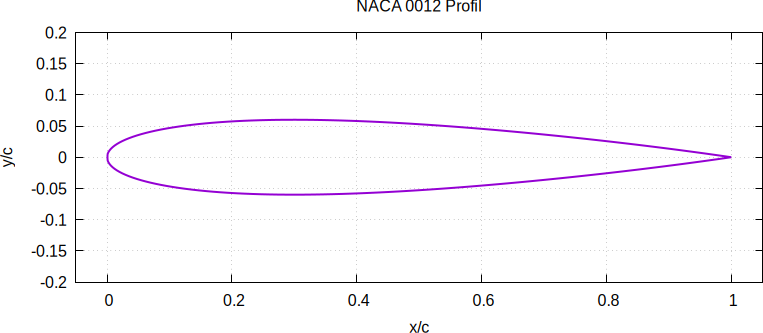
\includegraphics[width=\textwidth]{crop_004.png}
  \end{minipage}\hfill
  \begin{minipage}[t]{0.58\textwidth}
    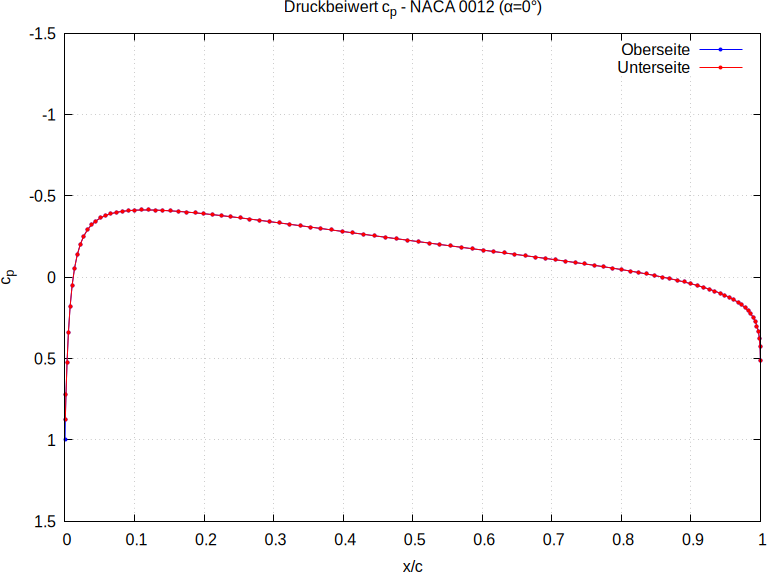
\includegraphics[width=\textwidth]{crop_007.png}
  \end{minipage}
  \vspace{-1mm}
  {\tiny\centering NACA\,0012: symmetrisch $\to$ $c_a\!=\!0$\par}
  \vspace{1.5mm}
  \begin{minipage}[t]{0.38\textwidth}
    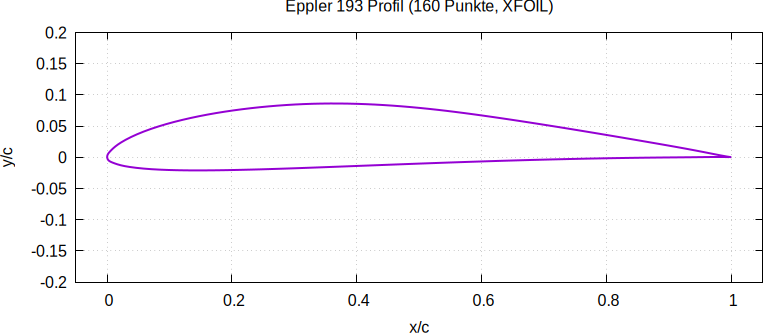
\includegraphics[width=\textwidth]{crop_002.png}
  \end{minipage}\hfill
  \begin{minipage}[t]{0.58\textwidth}
    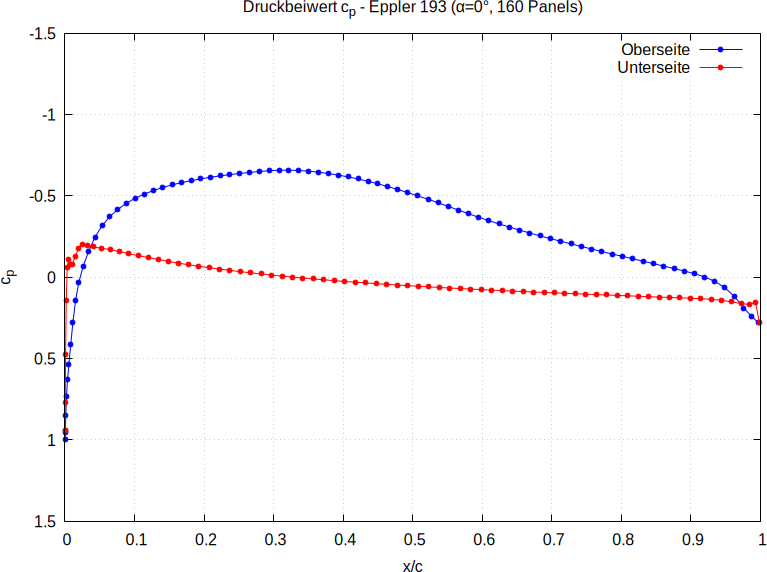
\includegraphics[width=\textwidth]{crop_008.png}
  \end{minipage}
  \vspace{-1mm}
  {\tiny\centering Eppler\,193: gewölbt $\to$ $c_a\!=\!0{,}378$\par}
\end{column}
\end{columns}

\end{frame}

%=== FOLIE 10: XFOIL-Validierung ===
\begin{frame}{Validierung mit XFOIL}
\footnotesize

\begin{columns}[T]
\begin{column}{0.57\textwidth}
Referenz: \textbf{XFOIL} (M.~Drela, MIT) -- Panelmethode mit
\emph{linear variierender} Wirbelbelegung.

\smallskip
\textbf{NACA\,0012} -- Abweichung $< 0{,}15\,\%$:

\vspace{1mm}
{\scriptsize
\begin{tabular}{@{}cccc@{}}
  \toprule
  $\alpha$ & $c_a$ (H-S) & $c_a$ (XFOIL) & Abw. \\
  \midrule
  $0^\circ$  & 0{,}0000 & 0{,}0000 & --      \\
  $5^\circ$  & 0{,}6027 & 0{,}6033 & 0{,}11\,\% \\
  $10^\circ$ & 1{,}2007 & 1{,}2020 & 0{,}11\,\% \\
  \bottomrule
\end{tabular}}

\smallskip
\textbf{Eppler-Profile} -- Abweichung 4--10\,\%:
\begin{itemize}\setlength\itemsep{0pt}
  \item H-S: \emph{konstante} Singularitäten pro Panel
  \item XFOIL: \emph{linear variierende} Wirbelbelegung
  \item Endliche Hinterkantendicke $\to$ Schließungspanel
\end{itemize}
\end{column}
\begin{column}{0.40\textwidth}
  \vspace{-1mm}
  \plotimg{crop_010.png}
  \vspace{-1mm}
  {\tiny\centering NACA\,0012: nahezu deckungsgleich\par}
  \vspace{2mm}
  \plotimg{crop_011.png}
  \vspace{-1mm}
  {\tiny\centering Eppler\,193: sichtbare Abweichung (4--8\,\%)\par}
\end{column}
\end{columns}

\end{frame}

%=== FOLIE 11: Zusammenfassung ===
\begin{frame}{Zusammenfassung}
\footnotesize

\begin{columns}[T]
\begin{column}{0.55\textwidth}
\textbf{Ergebnisse:}
\begin{itemize}\setlength\itemsep{3pt}
  \item Kreiszylinder: Konvergenz mit Ordnung $p\!=\!1$
  \item NACA\,0012 vs.\ XFOIL: $< 0{,}15\,\%$ Abweichung
  \item Eppler-Profile: 4--10\,\% Abweichung\\
        (konstante vs.\ lineare Wirbelbelegung,\\
        endliche Hinterkantendicke)
\end{itemize}
\end{column}
\begin{column}{0.42\textwidth}
\textbf{Rechenweg im Überblick:}

\medskip
\begin{enumerate}\setlength\itemsep{3pt}
  \item Annahmen $\to$ $\Delta\varphi = 0$
  \item Elementarlösung: $\varphi = \frac{m}{2\pi}\ln r$
  \item Quellverteilung auf Panels $\to$ Integrale $I,\,J$
  \item Undurchlässigkeit $\to$ $M\vec{q}=\vec{b}$
  \item $q_j$ bekannt $\to$ $v_{t,i}$ berechnen
  \item Bernoulli $\to$ $c_p = 1-(v_t/V_\infty)^2$
  \item Wirbelbelegung $\gamma$ + Kutta $\to$ $c_a$
\end{enumerate}
\end{column}
\end{columns}

\end{frame}

\end{document}
